\documentclass[aspectratio=169]{beamer}

\usepackage[utf8]{inputenc}
\usepackage[T1]{fontenc}
\usepackage{lmodern}
\usepackage{graphicx}
\usepackage{booktabs}

\usetheme{Madrid}
\setbeamertemplate{navigation symbols}{}
\setbeamertemplate{footline}[frame number]

\title[TETHER]{ARGOS Weekly Update}
\subtitle{TETHER: Causal Temporal Refinement for Frozen Surgical Stereo}
\author{Leonardo Pampaloni}
\institute{Aalborg University}
\date{\today}

\begin{document}

\begin{frame}
    \titlepage
\end{frame}

% ------------------------------------------------------------
\begin{frame}{The Setting}

\begin{columns}[T,totalwidth=\textwidth]

\begin{column}{0.53\textwidth}
\begin{block}{The question}
Can \emph{one} causal temporal module be trained once and attached,
unchanged, to heterogeneous \textbf{frozen} stereo estimators?
\end{block}

\vspace{0.6em}

\begin{block}{Constraints we accept}
\begin{itemize}
    \item No backbone internals.
    \item No future frames.
    \item Backbone weights never touched.
\end{itemize}
\end{block}
\end{column}

\begin{column}{0.43\textwidth}
\vspace{1.5em}
\begin{exampleblock}{The module}
\textbf{154{,}874} parameters.

\vspace{0.4em}
One scalar per pixel: how much to trust the past.
\end{exampleblock}
\end{column}

\end{columns}

\end{frame}

% ------------------------------------------------------------
\begin{frame}{Architecture Overview}

\centering
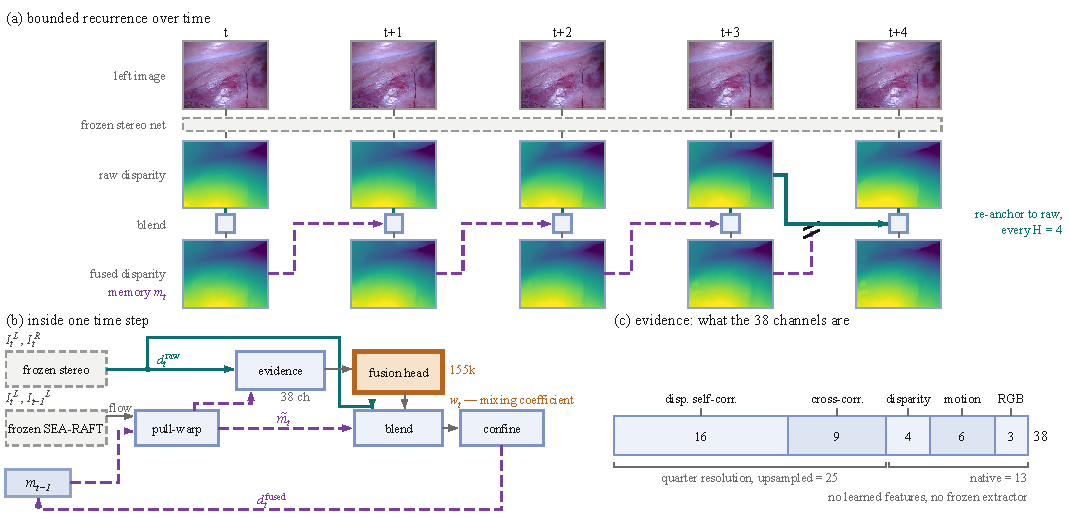
\includegraphics[width=0.97\textwidth]{figure_assets/Temporal_consistency_taxonomy.pdf}

\vspace{0.5em}
{\footnotesize Grey is frozen. \textbf{One orange block is trained.}
Memory is re-anchored to raw geometry every $H{=}4$ frames.}

\end{frame}

% ------------------------------------------------------------
\begin{frame}{It Transfers}

\begin{columns}[T,totalwidth=\textwidth]

\begin{column}{0.47\textwidth}

\begin{block}{Mean EPE reduction}
\centering
\begin{tabular}{lcc}
\toprule
Backbone $\rightarrow$ & seen & \textbf{unseen} \\
\midrule
SCARED-C D7 & $5.80\%$ & $4.79\%$ \\
DRENDS (\textbf{OOD}) & $5.57\%$ & $\mathbf{5.16\%}$ \\
\bottomrule
\end{tabular}

\vspace{0.4em}
{\footnotesize One frozen checkpoint everywhere. Bottom-right is the cell
usually left unevaluated.}
\end{block}

\vspace{0.4em}

\begin{block}{Against a published stabiliser}
\centering
\begin{tabular}{lccc}
\toprule
Method & Causal & EPE & Bad1 \\
\midrule
Raw & --- & $.3029$ & $2.09\%$ \\
BiDAStabilizer & \textbf{no} & $.3021$ & $1.99\%$ \\
\textbf{TETHER} & \textbf{yes} & $\mathbf{.2889}$ & $\mathbf{1.80\%}$ \\
\bottomrule
\end{tabular}
\end{block}

\end{column}

\begin{column}{0.49\textwidth}
\centering
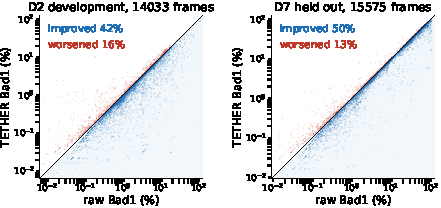
\includegraphics[width=\textwidth]{frame_scatter.pdf}

\vspace{0.4em}
{\footnotesize Every scored frame, all five backbones, no selection.
Below the diagonal is better.}
\end{column}

\end{columns}

\end{frame}

% ------------------------------------------------------------
\begin{frame}{Status}

\begin{block}{Paper}
Eight pages, one figure, three tables, everything else in a seven-page
supplement. Head-to-head comparison, three-seed study and the held-out
transfer matrix are in.
\end{block}

\vspace{0.6em}

\begin{block}{The ablations came back, and not the way we expected}
The learned feature extractor is not what makes the module work --- removing
it entirely is \emph{better} and eight times more stable across seeds, which
is why the shipped head is the smaller one. Relaxing the convex constraint
then beat the canonical model on the held-out endpoint, which under our
pre-registration means the claim that convexity explains cross-backbone
transfer has to be withdrawn. It is withdrawn. We do not know why the head
transfers.
\end{block}

\vspace{0.6em}

\begin{alertblock}{Running}
A $100$-epoch convergence probe against the locked $12$, to answer whether the
budget is a ceiling or a plateau. Not eligible for selection.
\end{alertblock}

\end{frame}

\end{document}
